% You should title the file with a .tex extension (hw1.tex, for example)
\documentclass[11pt]{article}

\usepackage{hyperref}
\usepackage{amsmath}
\usepackage{mathtools}
\usepackage{amssymb}
\usepackage{wrapfig}
\usepackage{fancyhdr}
\usepackage{tikz-qtree}
\usepackage{tikz-qtree-compat}
\usepackage[normalem]{ulem}
\usepackage{tikz}
\usepackage{systeme}
\usepackage{graphicx}
\DeclareMathOperator*{\argmin}{argmin}
\DeclareMathOperator*{\argmax}{argmax}

\oddsidemargin0cm
\topmargin-2cm     %I recommend adding these three lines to increase the 
\textwidth16.5cm   %amount of usable space on the page (and save trees)
\textheight23.5cm  

\newcommand{\question}[2] {\vspace{.25in} \hrule\vspace{0.5em}
\noindent{\bf #1: #2} \vspace{0.5em}
\hrule \vspace{.10in}}
\renewcommand{\part}[1] {\vspace{.10in} {\bf (#1)}}

\newcommand{\myname}{Sean Bittner}
\newcommand{\myandrew}{srb2201@columbia.edu}
\newcommand{\myhwnum}{12}

\setlength{\parindent}{0pt}
\setlength{\parskip}{5pt plus 1pt}
 
\DeclarePairedDelimiter\abs{\lvert}{\rvert}%
 %
\pagestyle{fancyplain}
\rhead{\fancyplain{}{\myname\\ \myandrew}}

\begin{document}

\medskip                        % Skip a "medium" amount of space
                                % (latex determines what medium is)
                                % Also try: \bigskip, \littleskip

\thispagestyle{plain}
\begin{center}                  % Center the following lines
{\Large Draft of new SC section} \\
Sean Bittner \\
November 4, 2020 \\
\end{center}

\section{Identifying neural mechanisms of flexible task switching} \label{results_SC}
In a rapid task switching experiment \cite{duan2015requirement}, rats were explicitly cued on each trial to either orient towards a visual stimulus in the Pro (P) task or orient away from a visual stimulus in the Anti (A) task (Fig. \ref{fig:SC}a). 
Neural recordings in the midbrain superior colliculus (SC) exhibited two populations of neurons that simultaneously represented both task context (Pro or Anti) and motor response (contralateral or ipsilateral to the recorded side): the Pro/Contra and Anti/Ipsi neurons \cite{duan2018collicular}.
Duan et al. proposed a model of SC that, like the V1 model analyzed in the previous section, is a four-population dynamical system.  
We analyzed this model, where the neuron-type populations are functionally-defined as the Pro- and Anti-populations in each hemisphere (left (L) and right (R)), their connectivity is parameterized geometrically  (Fig. \ref{fig:SC}B).
The input-output function of this model is chosen such that the population responses $x = [x_{LP}, x_{LA}, x_{RP}, x_{RA}]^\top$ are bounded from 0 to 1 giving rise to high (1) or low (0) responses at the end of the trial:
\begin{equation}
x_\alpha =\left(\frac{1}{2}\tanh\left(\frac{u_\alpha - \epsilon}{\zeta}\right)+ \frac{1}{2} \right)
\end{equation}
where $\epsilon = 0.05$ and $\zeta = 0.5$.  
The dynamics evolve with timescale $\tau=0.09$ via an internal variable $u$ governed by connectivity weights $W$
\begin{equation}
\tau \frac{du}{dt} = -u + Wx + h + \sigma dB
\end{equation}
with gaussian noise of variance $\sigma^2$ = 0.2.
The input $h$ is comprised of a cue-dependent input to the Pro or Anti populations, a stimulus orientation input to either the Left or Right populations, and a choice-period input to the entire network (see Section \ref{methods_SC}).
Here, we use EPI to determine the changes in network connectivity $z = [sW, vW, dW, hW]^{\top}$ resulting in greater levels of rapid task switching accuracy.

\begin{figure}
\begin{center}
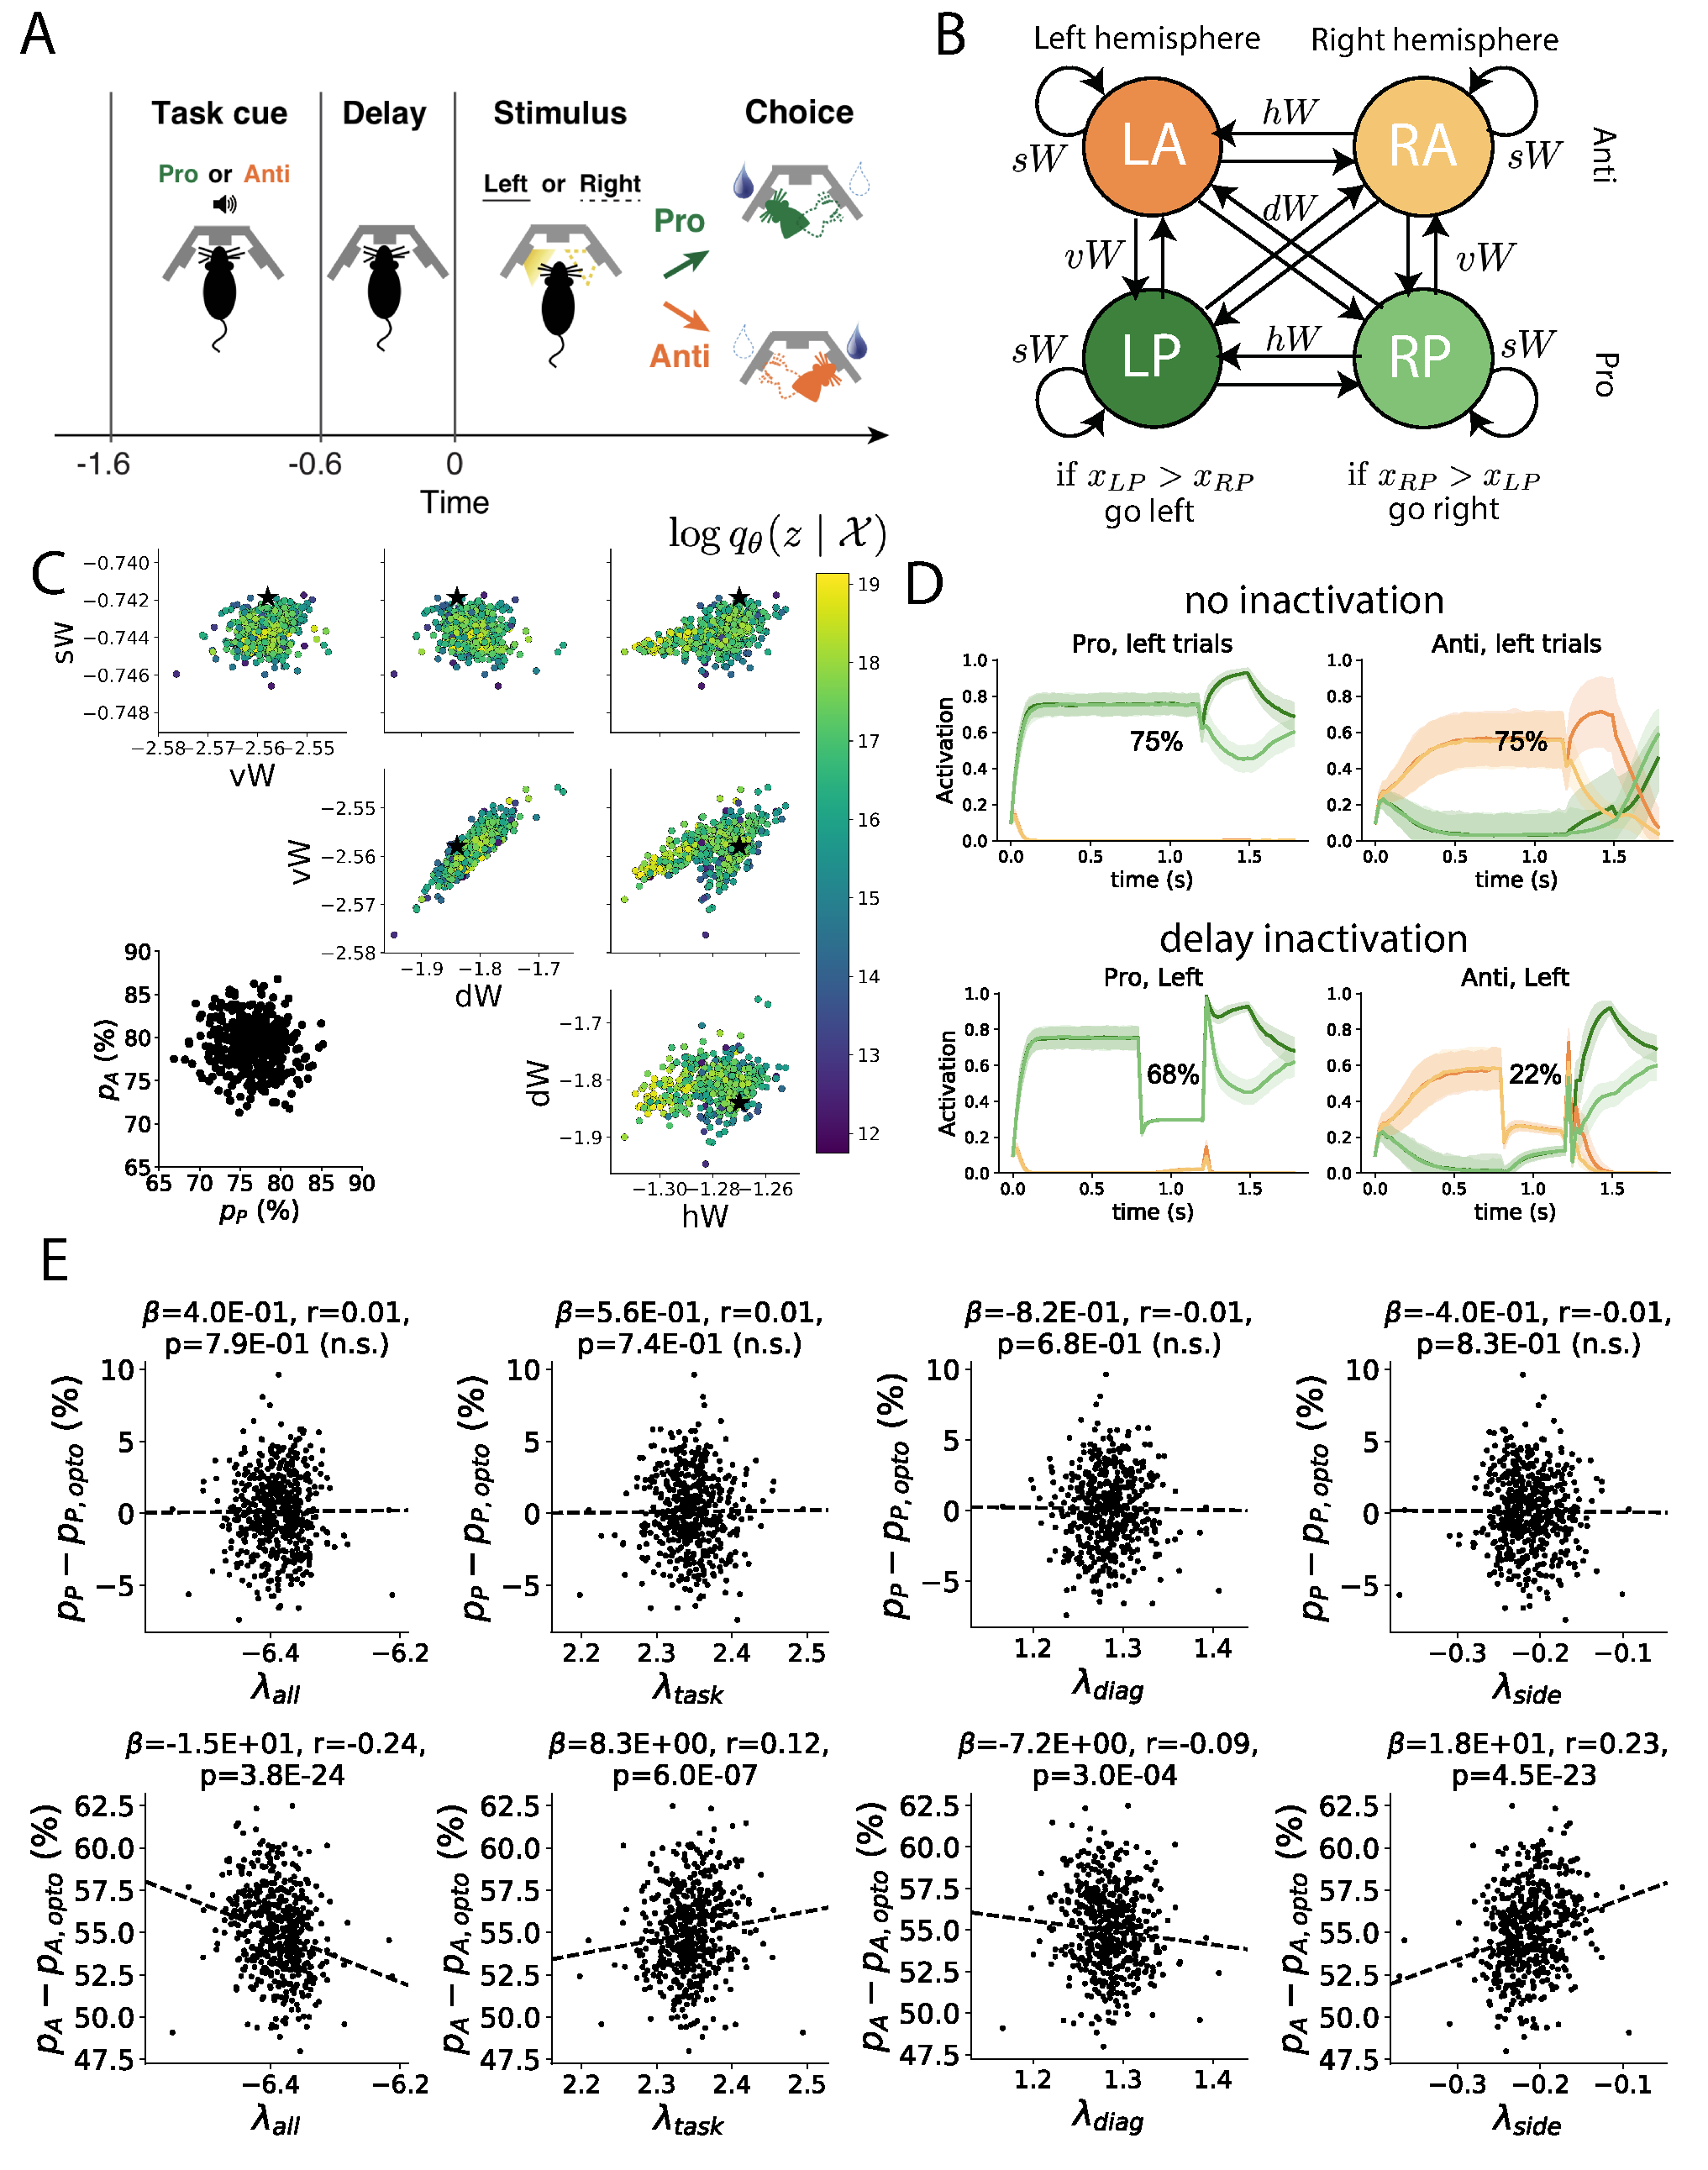
\includegraphics[scale=0.5]{figs/fig4.pdf}
\end{center}
\caption{\small EPI reveals changes in SC \cite{duan2018collicular} connectivity that control task accuracy.  
A. Rapid task switching behavioral paradigm (see text). 
B. Model of superior colliculus (SC). Neurons: LP - left pro, RP - right pro, LA - left anti, RA - right anti. 
Parameters: $sW$ - self, $hW$ - horizontal, $vW$ -vertical, $dW$ - diagonal weights.  
Subscripts $P$ and $A$ of connectivity weights indicate Pro or Anti populations, and e.g. $vW_{PA}$ is a vertical weight from an Anti to a Pro population.  
C. The Schur decomposition of the weight matrix $W = V\Lambda V^{-1}$ is a unique decomposition with orthogonal $V$ and upper triangular $\Lambda$. Schur modes: $v_{\text{all}}$, $v_{\text{task}}$, $v_{\text{side}}$, and $v_{\text{diag}}$.  
D. The marginal EPI distributions of the Schur eigenvalues at each level of task accuracy.
E. The correlation of Schur eigenvalue with task performance in each learned EPI distribution.}
\label{fig:SC}
\end{figure}

To quantify the emergent property of rapid task switching , we considered the requirements of this model in this behavioral paradigm.
At the end of successful trials, the response of the Pro population in the hemisphere of the correct choice must be greater than the Pro population in the opposite hemisphere.
Thus, we can formulate rapid task switching accuracy as the average number of successful trials over gaussian noise.
\begin{equation}
\mathcal{B}(p) ~~\triangleq~~ \mathbb{E}\begin{bmatrix} \hat{p}_P \\ \hat{p}_A \\ (\hat{p}_P-p)^2 \\ (\hat{p}_A - p)^2 \\ \sigma^2_{P,err} \\ \sigma^2_{A,err} \\ d_P \\ d_A \end{bmatrix} = \begin{bmatrix} p \\ p \\ 0.15^2 \\ 0.15^2 \\ 0 \\ 0 \\ 1 \\ 1 \end{bmatrix}.
\end{equation}
Thus, $\mathcal{B}(p)$ denotes Bernoulli, winner-take-all responses between Pro neurons in a model executing rapid task switching near accuracy level $p$.

We used EPI to learn distributions of the SC weight matrix parameters $z$ conditioned on of various levels of rapid task switching accuracy $\mathcal{B}(p)$ for $p \in \{50\%, 60\%, 70\%, 80\%, 90\%\}$.
To make sense of these inferred distributions, we followed the approach of Duan et al. by decomposing the connectivity matrix $W = V\Lambda V^{-1}$ in such a way (the Schur decomposition) that the basis vectors $v_i$ are the same for all $W$ (Fig. \ref{fig:SC}C). 
These basis vectors have intuitive roles in processing for this task, and are accordingly named the \textit{all} mode - all neurons co-fluctuate, \textit{side} mode - one side dominates the other, \textit{task} mode - the Pro or Anti populations dominate the other, and \textit{diag} mode - Pro- and Anti-populations of opposite hemispheres dominate the opposite pair. 
The corresponding eigenvalues (e.g. $\lambda_{\text{task}}$, which change according to $W$) indicate the degree to which activity along that mode is increased or decreased by $W$. 

We found that for greater task accuracies, the task mode eigenvalue increases, indicating the importance of $W$ to the task representation (Fig. \ref{fig:SC}D, purple; adjacent distributions from 60\% to 90\% have  $p<10^{-4}$, Mann-Whitney test with 50 estimates and 100 samples).
Stepping from random chance (50\%) networks to marginally task-performing (60\%) networks, there is a marked decrease of the side mode eigenvalues (Fig. \ref{fig:SC}D, orange; $p<10^{-4}$).  
Such side mode suppression relative to $50\%$ remains in the models achieving greater accuracy, revealing its importance towards task performance.
There were no interesting trends with task accuracy in the all or diag mode (hence not shown in Fig. \ref{fig:SC}). 
Importantly, we can conclude from our methodology that side mode suppression in $W$ allows rapid task switching, and that greater task-mode representations in $W$ increase accuracy.  
These hypotheses are confirmed by forward simulation of the SC model (Fig. \ref{fig:SC}E, see Section \ref{methods_SC}) suggesting experimentally testable predictions: increase in rapid task switching performance should be correlated with changes in effective connectivity corresponding to an increase in task mode and decrease in side mode eigenvalues.

\section{Supplementary}\label{methods_SC}
In the model of Duan et al \cite{duan2018collicular}, there are four total units: two in each hemisphere corresponding to the Pro/Contra and Anti/Ipsi populations.  
They are denoted as left Pro (LP), left Anti (LA), right Pro (RP) and right Anti (RA).  
Each unit has an activity ($x_\alpha$) and internal variable ($u_\alpha$) related by
\begin{equation}
x_\alpha =\left(\frac{1}{2}\tanh\left(\frac{u_\alpha - \epsilon}{\zeta}\right)+ \frac{1}{2} \right)
\end{equation}
where $\alpha \in \{LP, LA, RA, RP\}$ $\epsilon = 0.05$ and $\zeta = 0.5$ control the position and shape of the nonlinearity, respectively.

We order the elements of $x$ and $u$ in the following manner
\begin{equation}
x = \begin{bmatrix} x_{LP} \\ x_{LA} \\ x_{RP} \\ x_{RA} \end{bmatrix} \hspace{2cm} u = \begin{bmatrix} u_{LP} \\ u_{LA} \\ u_{RP} \\ u_{RA} \end{bmatrix}.
\end{equation}

 The internal variables follow dynamics:
\begin{equation}
\tau \frac{du}{dt} = -u + Wx + h + \sigma dB
\end{equation}
with time constant $\tau = 0.09s$ and Gaussian noise $\sigma dB$ controlled by the magnitude of $\sigma=1.0$.  The weight matrix has 8 parameters $sW_P$, $sW_A$, $vW_{PA}$, $vW_{AP}$, $hW_P$, $hW_A$, $dW_{PA}$, and $dW_{AP}$ (Fig. 4B):
\begin{equation}
W = \begin{bmatrix} sW_P & vW_{PA} & hW_P & dW_{PA}  \\ vW_{AP}  & sW_A & dW_{AP}  & hW_A \\ hW_P & dW_{PA}  & sW_P & vW_{PA}  \\ dW_{AP}  & hW_A & vW_{AP}  & sW_A \end{bmatrix}.
\end{equation}

The system receives five inputs throughout each trial, which has a total length of 1.8s.
\begin{equation}
h = h_{\text{rule}} + h_{\text{choice-period}} + h_{\text{light}}.
\end{equation}

There are rule-based inputs depending on the condition,
\begin{equation}h_{\text{P,rule}}(t) = \begin{cases}
                           I_{\text{P,rule}} [1, 0, 1, 0]^\top,& \text{if } t\leq 1.2s \\
                            0,              & \text{otherwise}
                         \end{cases}
\end{equation}
\begin{equation} h_{\text{A,rule}}(t) = \begin{cases}
                           I_{\text{A,rule}} [0, 1, 0, 1]^\top,& \text{if } t\leq 1.2s \\
                            0,              & \text{otherwise}
                         \end{cases}
\end{equation}
a choice-period input,
\begin{equation} h_{\text{choice}}(t) = \begin{cases}
                           I_{\text{choice}} [1, 1, 1, 1]^\top,& \text{if } t > 1.2s \\
                            0,              & \text{otherwise}
                         \end{cases}
\end{equation}
and an input to the right or left-side depending on where the light stimulus is delivered.     
\begin{equation}  h_{\text{light}}(t) = \begin{cases}
                           I_{\text{light}} [1, 1, 0, 0]^\top,& \text{if } t > 1.2s \text{ and Left} \\
                           I_{\text{light}} [0, 0, 1, 1]^\top,& \text{if } t > 1.2s \text{ and Right} \\
                            0,              & t \leq 1.2s
                         \end{cases} .
\end{equation}
The input parameterization was fixed to $I_{\text{P,rule}} = 10 $,  $I_{\text{A,rule}} = 10$,  $I_{\text{choice}} = 2$,  and $I_{\text{light}} = 1$.

To produce an accuracy rate of $p_{LP}$ in the Left, Pro condition, let $\hat{p}_i$ be the empirical average steady state response (final $x_{LP}$ at end of task) over M=500 Gaussian noise draws for a given SC model parameterization $z_i$:
\begin{equation}
 \hat{p}_i = \mathbb{E}_{\sigma dB} \left[ x_{LP} \mid s=L, c=P, z=z_i \right] = \frac{1}{M}\sum_{j=1}^M x_{LP}(s=L, c=P, z=z_i, \sigma dB_j)
 \end{equation}
 where stimulus $s \in \{L, R\}$, cue $c \in \{P, A\}$, and $\sigma dB_j$ is the Gaussian noise on trial $j$.
As with the V1 model, we only consider steady state responses of $x$, so $x_\alpha$ is used from here on to denote the steady state activity at the end of the trial.
For the first emergent property statistic, the average over EPI samples (from $q_\theta(z)$) is set to the desired value $p_{LP}$:
\begin{equation}
\mathbb{E}_{z_i \sim q_\phi} \left[ \mathbb{E}_{\sigma dB} \left[ x_{LP,\text{ss}} \mid s=L, c=P, z=z_i \right] \right] = \mathbb{E}_{z_i \sim q_\phi} \left[ \hat{p}_i \right] = p_{LP}.
\end{equation}

For the next emergent property statistic, we ask that the variance of the steady state responses across Gaussian draws, is the Bernoulli variance for the empirical rate $\hat{p}_i$:
\begin{equation}
\mathbb{E}_{z \sim q\phi} \left[ \sigma^2_{err} \right] = 0
\end{equation}
where the Bernoulli variance error $\sigma^2_{err}$ for the Pro task, left condition is
\begin{equation}
\sigma^2_{err} = Var_{\sigma dB} \left[ x_{LP} \mid s=L, c=P, z=z_i \right] - \hat{p}_i(1 - \hat{p}_i).
\end{equation}

We have an additional constraint that the Pro neuron on the opposite hemisphere should have the opposite value (0 and 1).  We can enforce this with another constraint:
\begin{equation}
\mathbb{E}_{z \sim q\phi} \left[ d_P \right] = 1,
\end{equation}
where the distance between Pro neuron steady states $d_P$ in the Pro condition is
\begin{equation}
d_P =  \mathbb{E}_{\sigma dB} \left[ (x_{LP} - x_{RP})^2  \mid s=L, c=P, z=z_i \right]
\end{equation}
The emergent property statistics only need to be measured during the Left stimulus condition of the Pro and Anti tasks, since the network is symmetrically parameterized.
In total, the emergent property of rapid task switching at accuracy level $p$ was defined as
\begin{equation}
\mathcal{B}(p) ~~\triangleq~~ \mathbb{E}\begin{bmatrix} \hat{p}_P \\ \hat{p}_A \\ (\hat{p}_P-p)^2 \\ (\hat{p}_A - p)^2 \\ \sigma^2_{P,err} \\ \sigma^2_{A,err} \\ d_P \\ d_A \end{bmatrix} = \begin{bmatrix} p \\ p \\ 0.15^2 \\ 0.15^2 \\ 0 \\ 0 \\ 1 \\ 1 \end{bmatrix}.
\end{equation}

Since the maximum variance of a random variable bounded from 0 to 1 is the Bernoulli variance $\hat{p}(1-\hat{p})$, and the maximum squared difference between to variables bounded from 0 to 1 is 1, we do not need to control the second moment of these test statistics. 
These variables are dynamical system states and can only exponentially decay (or saturate) to 0 (or 1), so the Bernoulli variance error and squared difference constraints cannot be satisfied exactly in simulation.  
This is important to be mindful of when evaluating the convergence criteria.  
Instead of using our usual hypothesis testing criteria for convergence to the emergent property, we set a slack variable threshold only for these technically infeasible emergent property values to 0.05.

Using EPI to learn distributions of dynamical systems producing Bernoulli responses at a given rate (with small variance around that rate) was more challenging than expected.  
There is a pathology in this optimization setup, where the learned distribution of weights is bimodal attributing a fraction $p$ of the samples to an expansive mode (which always sends $x_{LP}$ to 1), and a fraction $1-p$ to a decaying mode (which always sends $x_{LP}$ to 0).  
This pathology was avoided using an inequality constraint prohibiting parameter samples that resulted in low variance of responses across noise.


\begin{table}[h]
\begin{tabular}{l|l|l|l|l}
$\lambda$  & $\hat{p}$ & $q_\theta(z)$ & $r$ & p-value \\ \hline
$\lambda_{\text{task}}$ & $\hat{p}_P$ & $q(z \mid \mathcal{B}(60\%))$ & $1.24 \times 10^{-01}$ & $p<10^{-4}$  \\ \hline
$\lambda_{\text{task}}$ & $\hat{p}_P$ & $q(z \mid \mathcal{B}(70\%))$ & $7.56 \times 10^{-01}$ & $p<10^{-4}$ \\ \hline
$\lambda_{\text{task}}$ & $\hat{p}_P$ & $q(z \mid \mathcal{B}(80\%))$ & $4.59 \times 10^{-01}$ & $p<10^{-4}$  \\ \hline
$\lambda_{\text{task}}$ & $\hat{p}_P$ & $q(z \mid \mathcal{B}(90\%))$ & $3.76 \times 10^{-01}$ & $p<10^{-4}$  \\ \hline

$\lambda_{\text{task}}$ & $\hat{p}_A$ & $q(z \mid \mathcal{B}(60\%))$ & $4.80 \times 10^{-02}$ & $p<.01$ \\ \hline
$\lambda_{\text{task}}$ & $\hat{p}_A$ & $q(z \mid \mathcal{B}(70\%))$ & $2.08 \times 10^{-01}$ & $p<10^{-4}$  \\ \hline
$\lambda_{\text{task}}$ & $\hat{p}_A$ & $q(z \mid \mathcal{B}(80\%))$ & $4.84 \times 10^{-01}$ & $p<10^{-4}$  \\ \hline
$\lambda_{\text{task}}$ & $\hat{p}_A$ & $q(z \mid \mathcal{B}(90\%))$ & $4.25 \times 10^{-01}$ & $p<10^{-4}$  \\ \hline

$\lambda_{\text{side}}$ & $\hat{p}_P$ & $q(z \mid \mathcal{B}(50\%))$ & $-7.57 \times 10^{-02}$ & $p<10^{-4}$  \\ \hline
$\lambda_{\text{side}}$ & $\hat{p}_P$ & $q(z \mid \mathcal{B}(60\%))$ & $-6.73 \times 10^{-02}$ & $p<10^{-4}$  \\ \hline
$\lambda_{\text{side}}$ & $\hat{p}_P$ & $q(z \mid \mathcal{B}(70\%))$ & $-4.86 \times 10^{-01}$ & $p<10^{-4}$  \\ \hline
$\lambda_{\text{side}}$ & $\hat{p}_P$ & $q(z \mid \mathcal{B}(80\%))$ & $-1.43 \times 10^{-01}$ & $p<10^{-4}$  \\ \hline
$\lambda_{\text{side}}$ & $\hat{p}_P$ & $q(z \mid \mathcal{B}(90\%))$ & $-1.93 \times 10^{-01}$ & $p<10^{-4}$  \\ \hline

$\lambda_{\text{side}}$ & $\hat{p}_A$ & $q(z \mid \mathcal{B}(60\%))$ & $-7.60 \times 10^{-02}$ & $p<10^{-4}$  \\ \hline
$\lambda_{\text{side}}$ & $\hat{p}_A$ & $q(z \mid \mathcal{B}(70\%))$ & $-2.73 \times 10^{-01}$ & $p<10^{-4}$  \\ \hline
$\lambda_{\text{side}}$ & $\hat{p}_A$ & $q(z \mid \mathcal{B}(80\%))$ & $-2.74 \times 10^{-01}$ & $p<10^{-4}$  \\ \hline
\end{tabular}
\caption{\small Table of significant correlation values from Fig. \ref{fig:SC}E.}
\end{table}

For each accuracy level $p$, we ran EPI for 10 different random seeds  using an architecture of 10 planar flows with a  support of $z \in \mathbb{R}^8$.   
We used an augmented Lagrangian coefficient of $c_0 = 10^2$, a batch size $n=300$, and set $\nu = 0.5$, and initialized $q_\theta(z)$ to produce an isotropic Gaussian of zero mean with standard deviation $\sigma_{\text{init}} = 1$.
The EPI distributions shown in Fig. \ref{fig:SC} are the converged distributions with maximum entropy across random seeds.

We report significant correlations $r$ and their p-values from Figure \ref{fig:SC}E in Table 1.  
Correlations were measured from 5,000 samples of $q_\theta(z \mid \mathcal{B}(p))$ and p-values are reported for one-tailed tests, since we hypothesized a positive correlation between task accuracies $p_P$ or $p_A$ and $\lambda_{\text{task}}$, and a negative correlation between task accuracies $p_P$ and $p_A$ and $\lambda_{\text{side}}$.

\bibliography{epi}
\bibliographystyle{unsrt}

\end{document}